\documentclass[tikz]{standalone}

\begin{document}
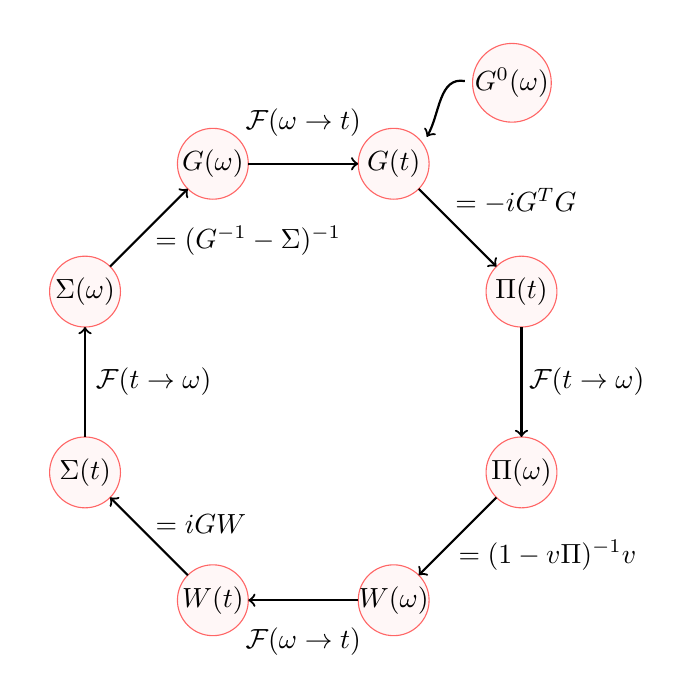
\begin{tikzpicture}
\clip (-3.5, -3.6) rectangle (4.5,4.5);
	


\filldraw[color=red!60, fill=red!3](2.77163859753386,1.1480502970952693) circle (0.45);
\node[] at (2.77163859753386, 1.1480502970952693) {$\Pi(t)$};


\filldraw[color=red!60, fill=red!3](1.1480502970952693,2.77163859753386) circle (0.45);
\node[] at (1.1480502970952693, 2.77163859753386) {$G(t)$};



\filldraw[color=red!60, fill=red!3](-1.1480502970952693,2.77163859753386) circle (0.45);
\node[] at (-1.1480502970952693, 2.77163859753386) {$G(\omega)$};


\filldraw[color=red!60, fill=red!3](-2.7716385975338595,1.1480502970952697) circle (0.45);
\node[] at (-2.7716385975338595, 1.1480502970952697) {$\Sigma(\omega)$};

\filldraw[color=red!60, fill=red!3](-2.7716385975338595,-1.1480502970952697) circle (0.45);
\node[] at (-2.7716385975338595, -1.1480502970952697) {$\Sigma(t)$};

\filldraw[color=red!60, fill=red!3](-1.1480502970952697,-2.771638597533859) circle (0.45);
\node[] at (-1.1480502970952697, -2.771638597533859) {$W(t)$};

\filldraw[color=red!60, fill=red!3](1.1480502970952697,-2.771638597533859) circle (0.45);
\node[] at (1.1480502970952697, -2.771638597533859) {$W(\omega)$};

\filldraw[color=red!60, fill=red!3](2.77163859753386,-1.1480502970952693) circle (0.45);
\node[] at (2.77163859753386, -1.1480502970952693) {$\Pi(\omega)$};


\node[rotate=0] at (2.7,2.3) {$=-iG^TG$};

\node[rotate=0] at (3.6,0) {$\mathcal{F}(t\to\omega)$};

\node[rotate=0] at (3.1,-2.2) {$=(1-v\Pi)^ {-1}v$};

\node[rotate=0] at (0,-3.3) {$\mathcal{F}(\omega\to t)$};

\node[rotate=0] at (-1.3,-1.8) {$=iGW$};

\node[rotate=0] at (-1.9,0) {$\mathcal{F}(t\to\omega)$};

\node[rotate=0] at (-0.7,1.8) {$=(G^{-1}-\Sigma)^ {-1}$};

\node[rotate=0] at (0,3.3) {$\mathcal{F}(\omega\to t)$};


\filldraw[color=red!60, fill=red!3](2.65,3.8) circle (0.5);
\node[] at (2.65,3.8) {$G^0(\omega)$};


\node[anchor=east] at (2.3,3.8) (a01pos) {};
\node[anchor=west] at (1.373,2.99) (a01) {};
\draw[thick, ->] (a01) edge[out=60,in=170,<-] (a01pos);

%\node[rotate=0] at (0,-2) {\footnotesize $\Pi = -iG\Gamma G$};

%\draw[->] (1.2,-0.01) arc (0:-180:1.2);
%\draw[->] (-1.2,0.01) arc (180:0:1.2);

\draw[thick, black, ->] (1.4662483486292157, 2.4534405459999133) -- (2.4534405459999133, 1.4662483486292157);
\draw[thick, black, <-] (2.771638597533859, -0.6980502970952702) -- (2.77163859753386, 0.6980502970952693);

\draw[thick, black, <-] (1.4662483486292144, -2.453440545999914)-- (2.4534405459999125, -1.4662483486292164);

\draw[thick, black, ->] (0.6980502970952682, -2.77163859753386) -- (-0.69805029709527, -2.771638597533859);

\draw[thick, black, <-] (-2.453440545999914, -1.4662483486292148) -- (-1.466248348629216, -2.4534405459999125);

\draw[thick, black, ->] (-2.771638597533859, -0.6980502970952702) -- (-2.77163859753386, 0.6980502970952693);

\draw[thick, black, <-] (-1.4662483486292157, 2.4534405459999133) -- (-2.4534405459999133, 1.4662483486292157);

\draw[thick, black, <-] (0.6980502970952682, 2.77163859753386) -- (-0.69805029709527, 2.771638597533859);


\end{tikzpicture}
\end{document}
